\documentclass[tikz,border=2pt]{standalone}
\usepackage{amsmath,amssymb}
\usepackage{tikz}
\usetikzlibrary{matrix,arrows.meta}

\begin{document}
% Final tableau of the Giapetto LP: every objective-row coefficient of a nonbasic variable
% is nonnegative (z + s_1 + s_2 = 180), so no variable can still improve z: optimal.
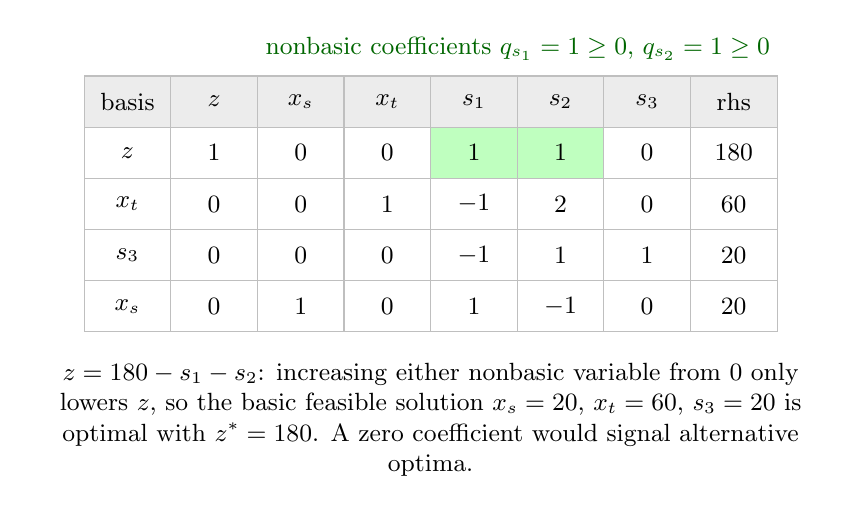
\begin{tikzpicture}[every node/.style={font=\small}, >={Latex[length=1.8mm]}]
	\matrix (T) [matrix of math nodes, nodes={minimum width=1.1cm, minimum height=6.5mm, anchor=center, draw=gray!50}, column sep=-\pgflinewidth, row sep=-\pgflinewidth] at (0,0) {
		|[fill=gray!15]| \text{basis} & |[fill=gray!15]| z & |[fill=gray!15]| x_s & |[fill=gray!15]| x_t & |[fill=gray!15]| s_1 & |[fill=gray!15]| s_2 & |[fill=gray!15]| s_3 & |[fill=gray!15]| \text{rhs} \\
		z & 1 & 0 & 0 & |[fill=green!25]| 1 & |[fill=green!25]| 1 & 0 & 180 \\
		x_t & 0 & 0 & 1 & -1 & 2 & 0 & 60 \\
		s_3 & 0 & 0 & 0 & -1 & 1 & 1 & 20 \\
		x_s & 0 & 1 & 0 & 1 & -1 & 0 & 20 \\
	};
	\node[green!40!black, anchor=south] at ([yshift=2pt]T-1-5.north east) {nonbasic coefficients $q_{s_1}=1\ge0$, $q_{s_2}=1\ge0$};
	\node[anchor=north, align=flush center, text width=10cm] at ([yshift=-4pt]T.south) {$z=180-s_1-s_2$: increasing either nonbasic variable from $0$ only lowers $z$, so the basic feasible solution $x_s=20$, $x_t=60$, $s_3=20$ is optimal with $z^\ast=180$. A zero coefficient would signal alternative optima.};
\end{tikzpicture}
\end{document}
